\section{Additional Benchmarks}
\label{sec:additional_benchmarks}

% \begin{figure}[!htb]
% \begin{tabular}{lll}
%   \includegraphics[height=0.16\textheight]{figures/ICLR_experiments/walltime_gpu_MIMO_10000_FTP.pdf} &   \includegraphics[height=0.16\textheight]{figures/ICLR_experiments/total_all_gflops_MIMO_10000_FTP.pdf} &  \includegraphics[height=0.16\textheight]{figures/ICLR_experiments/mean_all_gflops_MIMO_10000_FTP.pdf} \\
%   \includegraphics[height=0.16\textheight]{figures/ICLR_experiments/walltime_normalized_gpu_MIMO_10000_FTP.pdf} &   \includegraphics[height=0.16\textheight]{figures/ICLR_experiments/total_normalized_all_gflops_MIMO_10000_FTP.pdf} \\
% \end{tabular}
% \caption{Analysis of MIMO performance for different tensor products with Triton implementation on RTX A5500 : Total walltime (top row),  Total normalized walltime (second row), Total GFLOPs   (third row) and Total normalized GFLOPs (bottom row). Note that MTP only supports MIMO. We had to skip values due to profiling errors.}
% \label{experiments:benchmarking_gpu_ftp}
% \end{figure}

\begin{figure}[!htb]
\begin{tabular}{lll}
  
  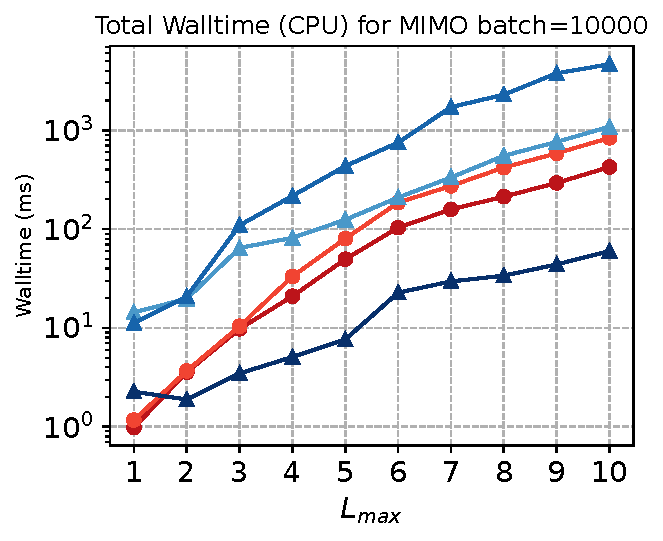
\includegraphics[height=0.16\textheight]{figures/ICLR_experiments/walltime_cpu_MIMO_10000.pdf} & 
  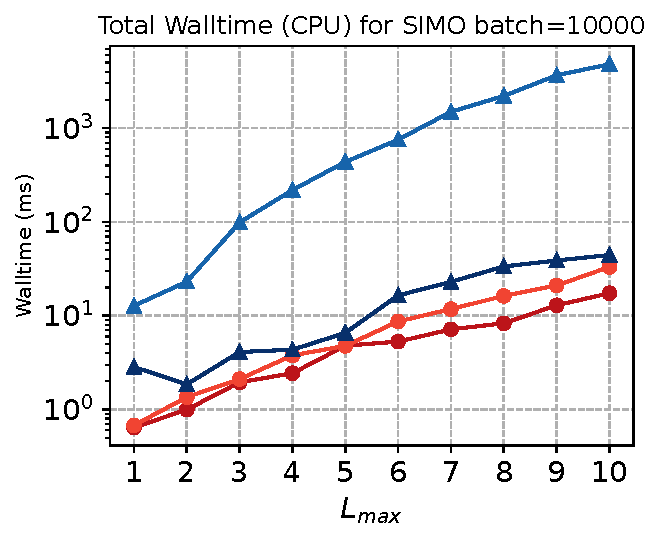
\includegraphics[height=0.16\textheight]{figures/ICLR_experiments/walltime_cpu_SIMO_10000.pdf} &  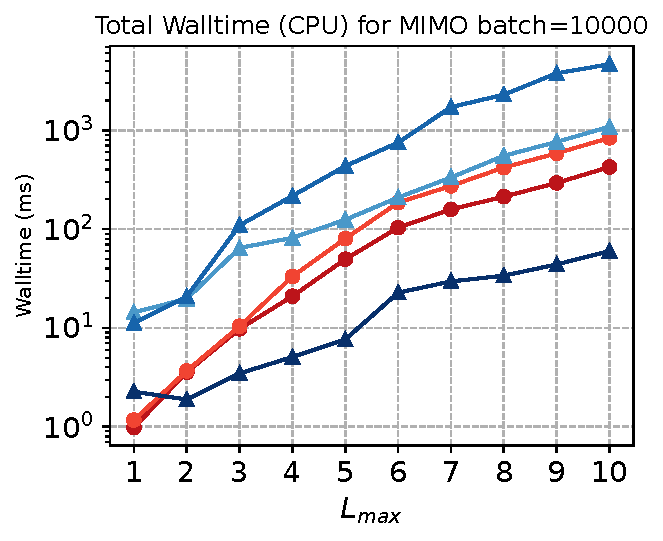
\includegraphics[height=0.16\textheight]{figures/ICLR_experiments/walltime_cpu_MIMO_10000.pdf} \\
  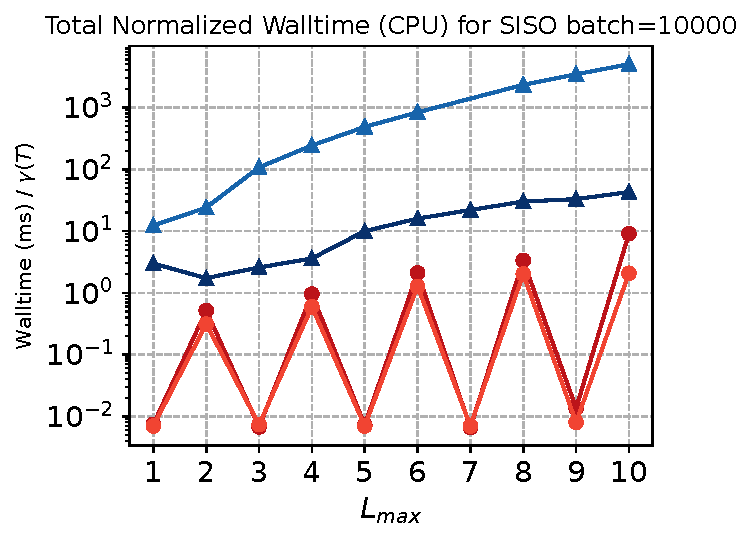
\includegraphics[height=0.16\textheight]{figures/ICLR_experiments/walltime_normalized_cpu_SISO_10000.pdf} &   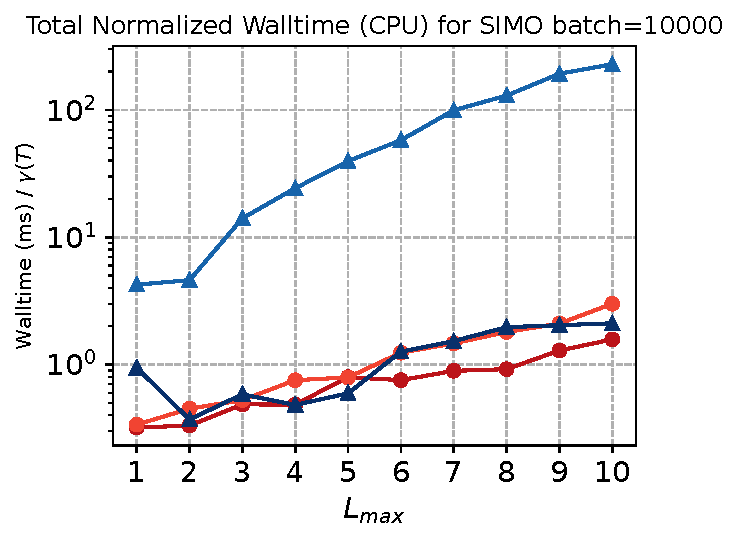
\includegraphics[height=0.16\textheight]{figures/ICLR_experiments/walltime_normalized_cpu_SIMO_10000.pdf} &  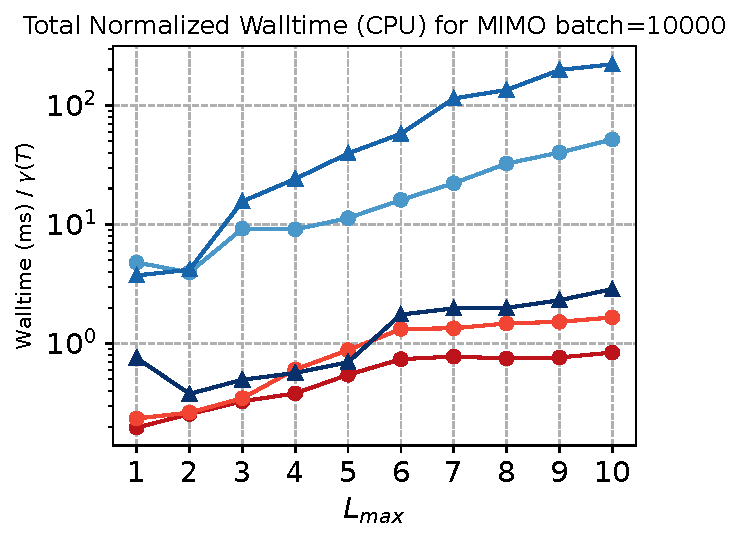
\includegraphics[height=0.16\textheight]{figures/ICLR_experiments/walltime_normalized_cpu_MIMO_10000.pdf} \\
  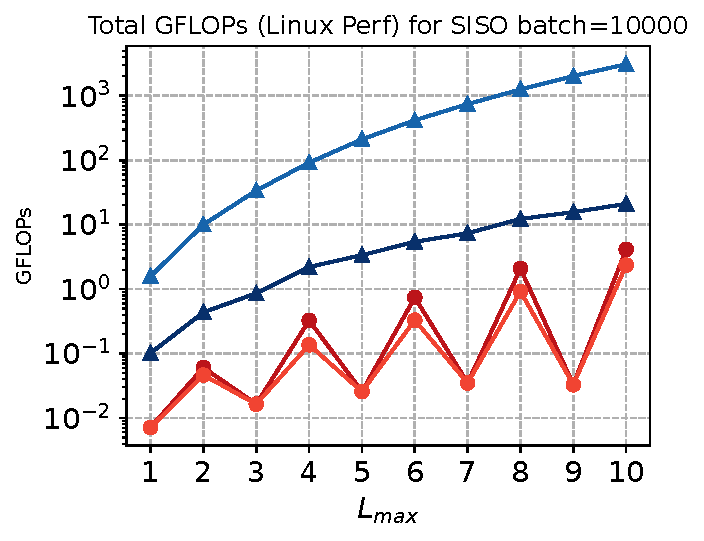
\includegraphics[height=0.16\textheight]{figures/ICLR_experiments/total_all_gflops_SISO_10000_cpu.pdf} &   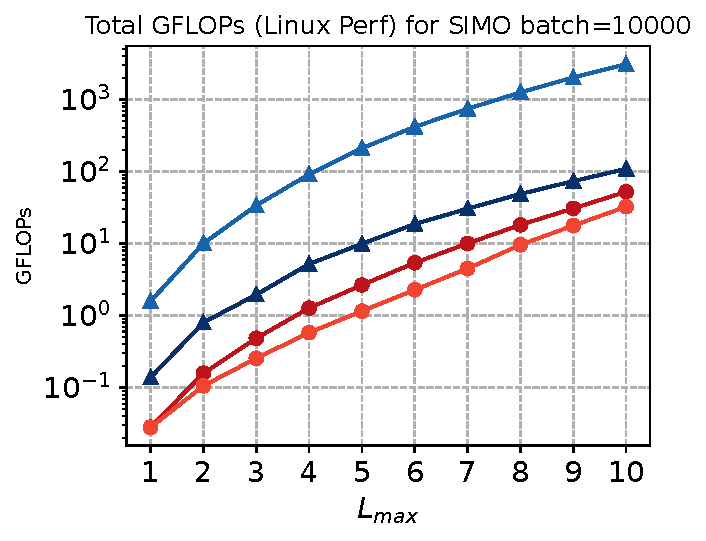
\includegraphics[height=0.16\textheight]{figures/ICLR_experiments/total_all_gflops_SIMO_10000_cpu.pdf} &  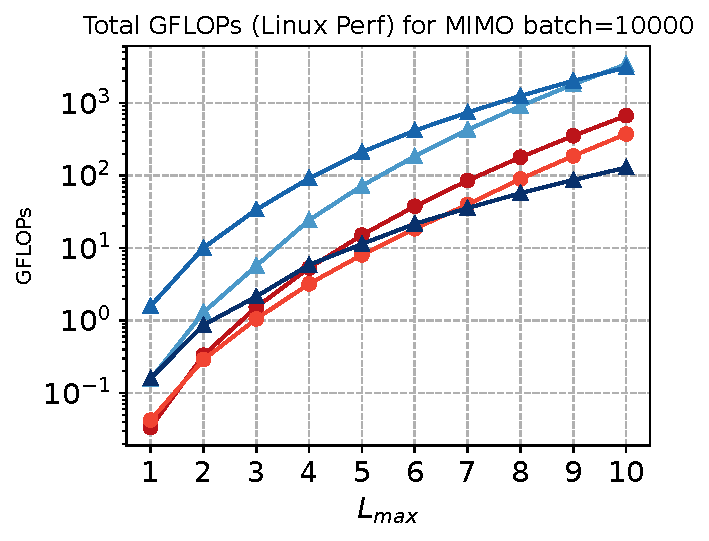
\includegraphics[height=0.16\textheight]{figures/ICLR_experiments/total_all_gflops_MIMO_10000_cpu.pdf} \\
  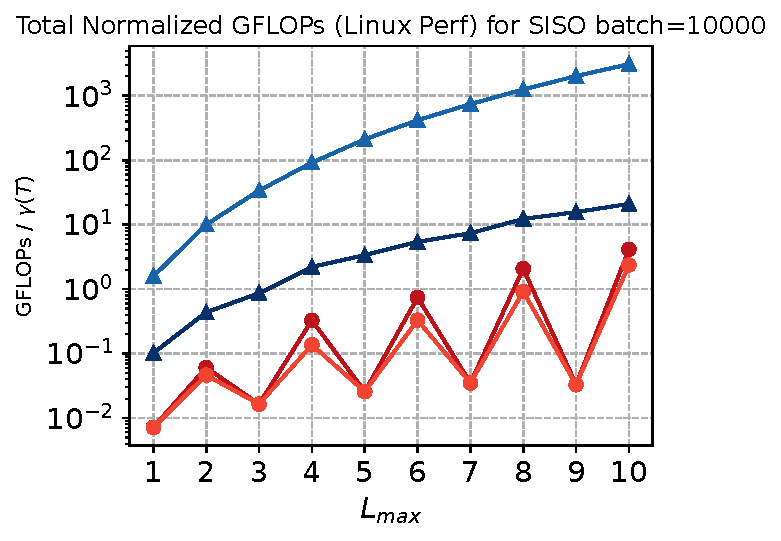
\includegraphics[height=0.16\textheight]{figures/ICLR_experiments/total_normalized_all_gflops_SISO_10000_cpu.pdf} &   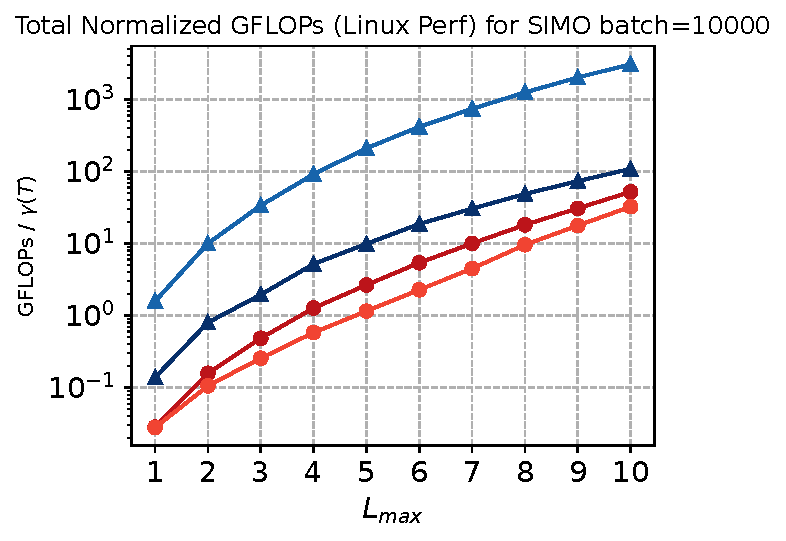
\includegraphics[height=0.16\textheight]{figures/ICLR_experiments/total_normalized_all_gflops_SIMO_10000_cpu.pdf} &  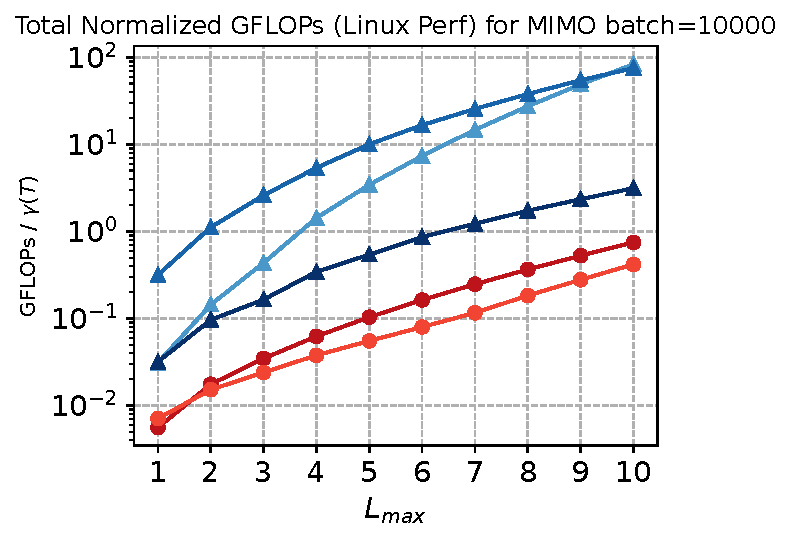
\includegraphics[height=0.16\textheight]{figures/ICLR_experiments/total_normalized_all_gflops_MIMO_10000_cpu.pdf} \\
\end{tabular}
\caption{Analysis of SISO, SIMO and MIMO (\autoref{tab:asymptotic_runtimes} for input settings) performance for different tensor products on AMD EPYC 7313 : Total walltime (top row),  Total normalized walltime (second row), Total GFLOPs   (third row) and Total normalized GFLOPs (bottom row). Note that MTP only supports MIMO. We had to skip values due to profiling errors.}
\label{experiments:benchmarking_cpu}
\end{figure}

\begin{figure}[!htb]
\begin{tabular}{lll}
  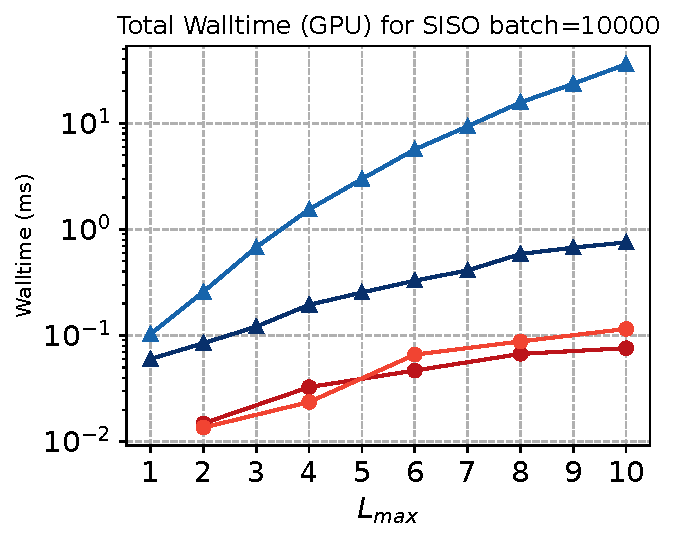
\includegraphics[height=0.16\textheight]{figures/ICLR_experiments/walltime_gpu_SISO_10000_RTX.pdf} &   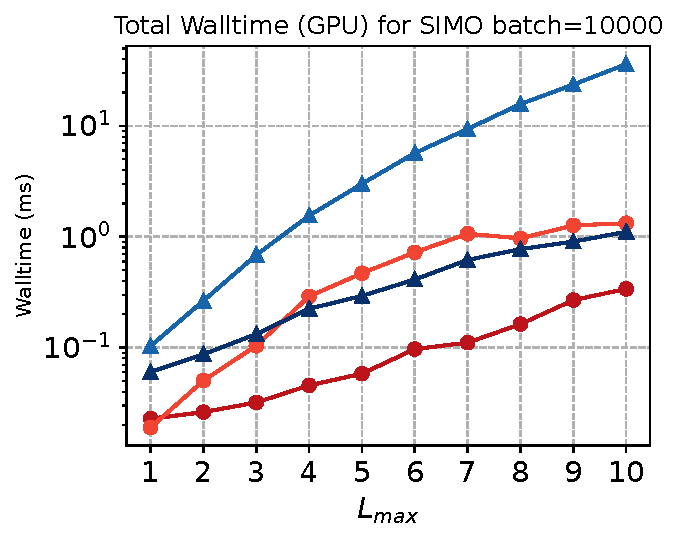
\includegraphics[height=0.16\textheight]{figures/ICLR_experiments/walltime_gpu_SIMO_10000_RTX.pdf} &  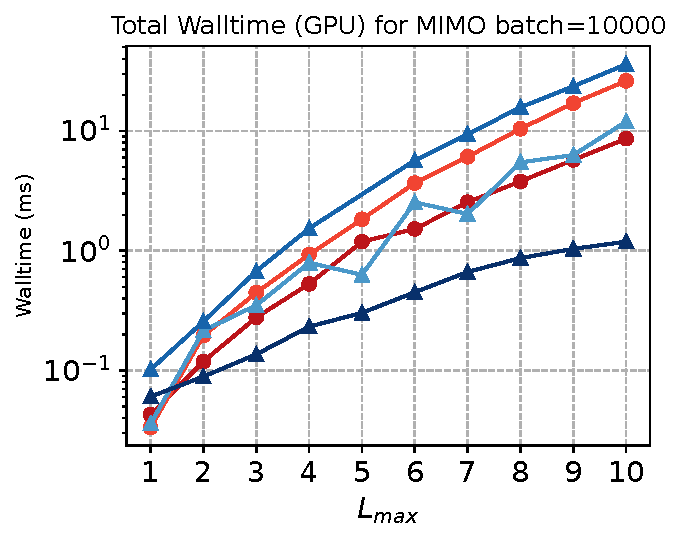
\includegraphics[height=0.16\textheight]{figures/ICLR_experiments/walltime_gpu_MIMO_10000_RTX.pdf} \\
  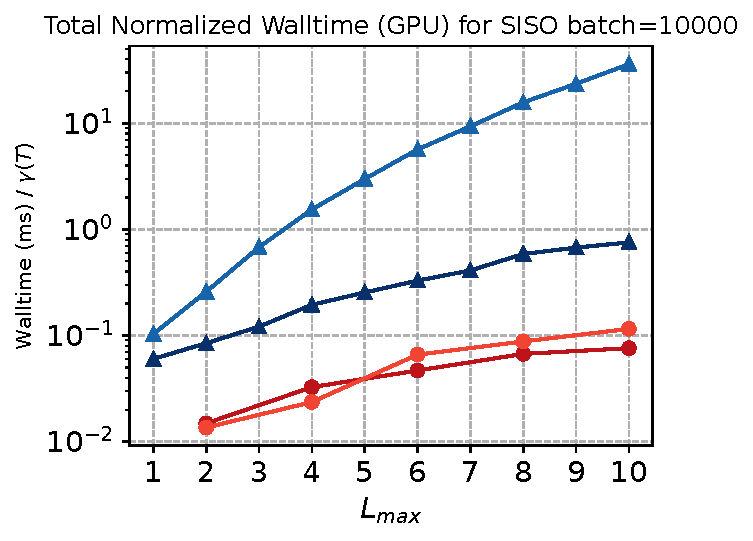
\includegraphics[height=0.16\textheight]{figures/ICLR_experiments/walltime_normalized_gpu_SISO_10000_RTX.pdf} &   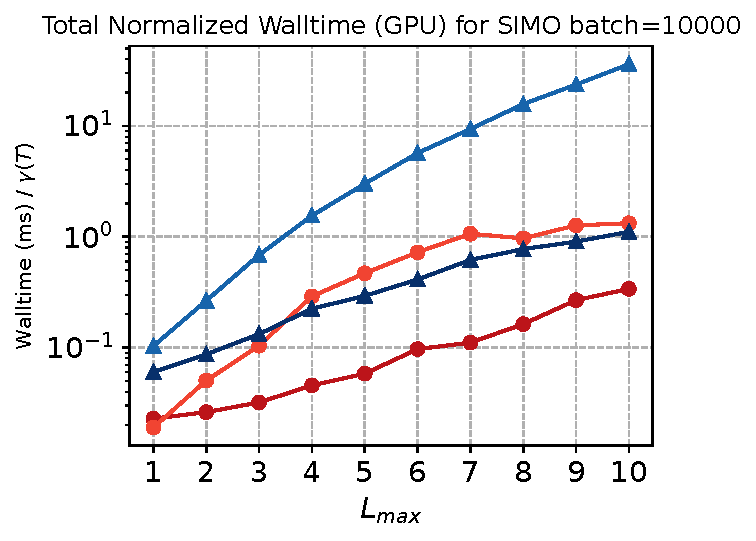
\includegraphics[height=0.16\textheight]{figures/ICLR_experiments/walltime_normalized_gpu_SIMO_10000_RTX.pdf} &  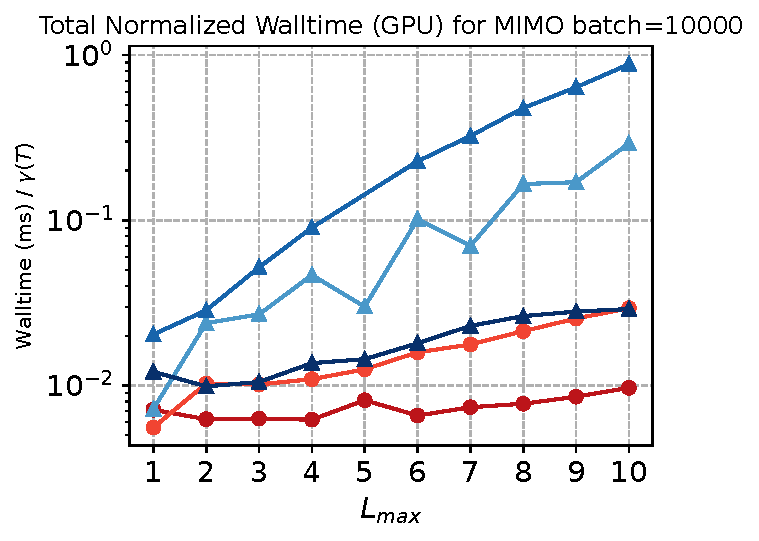
\includegraphics[height=0.16\textheight]{figures/ICLR_experiments/walltime_normalized_gpu_MIMO_10000_RTX.pdf} \\
  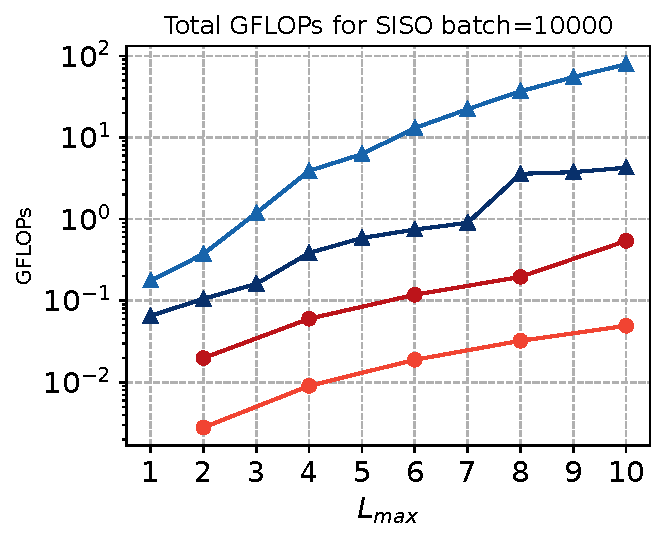
\includegraphics[height=0.16\textheight]{figures/ICLR_experiments/total_all_gflops_SISO_10000_RTX.pdf} &   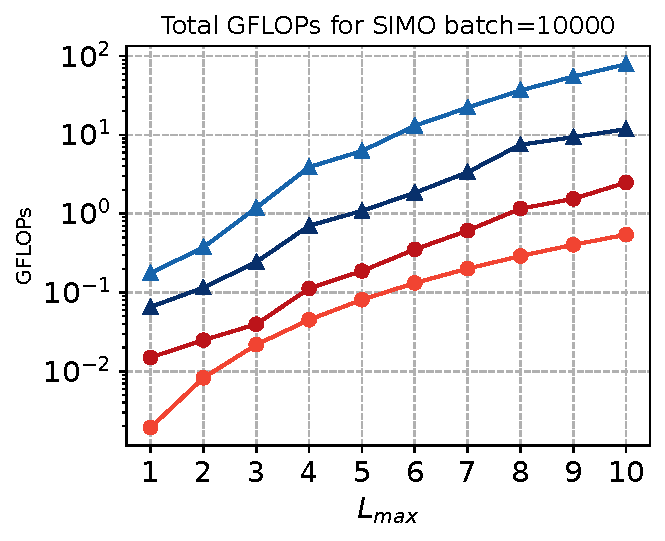
\includegraphics[height=0.16\textheight]{figures/ICLR_experiments/total_all_gflops_SIMO_10000_RTX.pdf} &  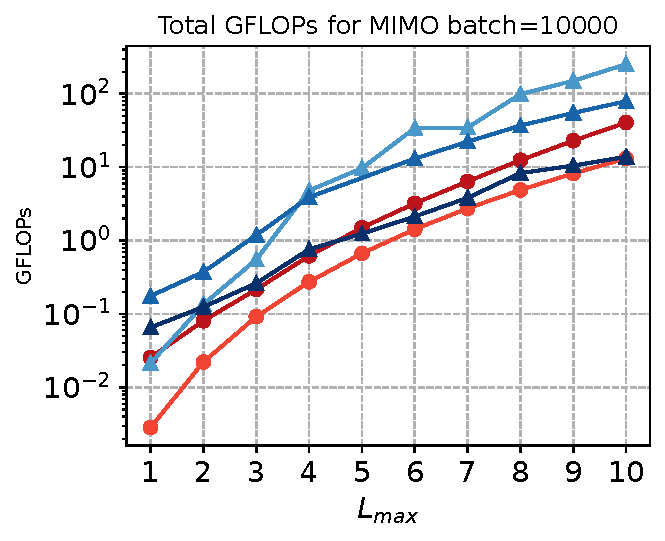
\includegraphics[height=0.16\textheight]{figures/ICLR_experiments/total_all_gflops_MIMO_10000_RTX.pdf} \\
  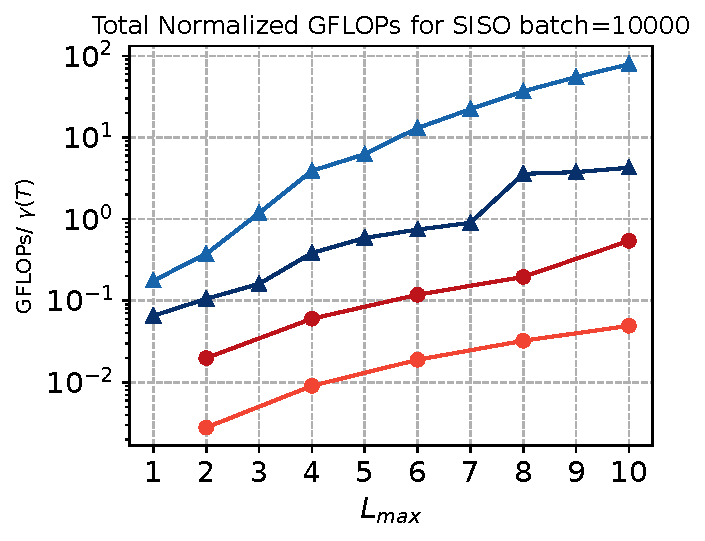
\includegraphics[height=0.16\textheight]{figures/ICLR_experiments/total_normalized_all_gflops_SISO_10000_RTX.pdf} &   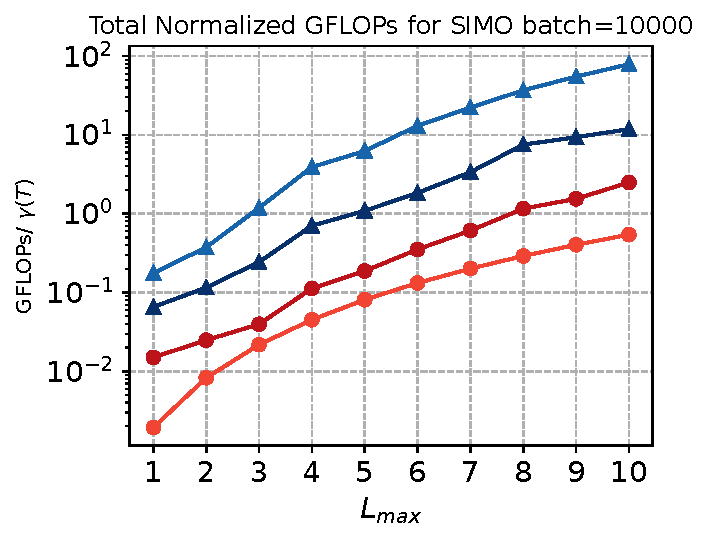
\includegraphics[height=0.16\textheight]{figures/ICLR_experiments/total_normalized_all_gflops_SIMO_10000_RTX.pdf} &  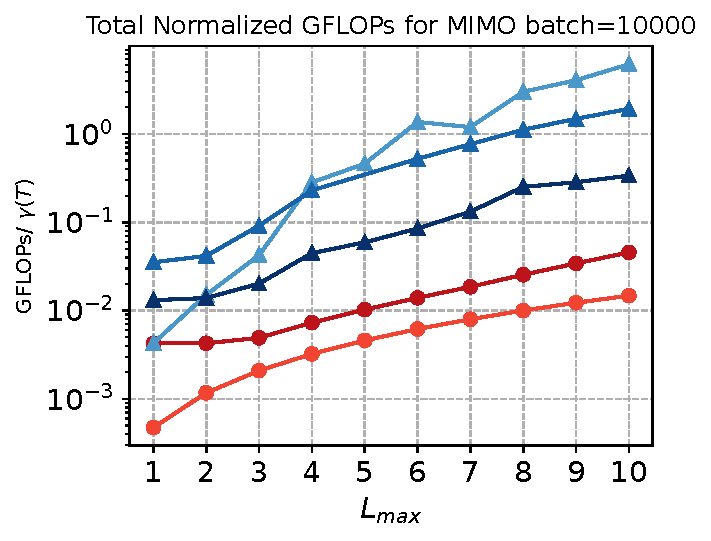
\includegraphics[height=0.16\textheight]{figures/ICLR_experiments/total_normalized_all_gflops_MIMO_10000_RTX.pdf} \\
  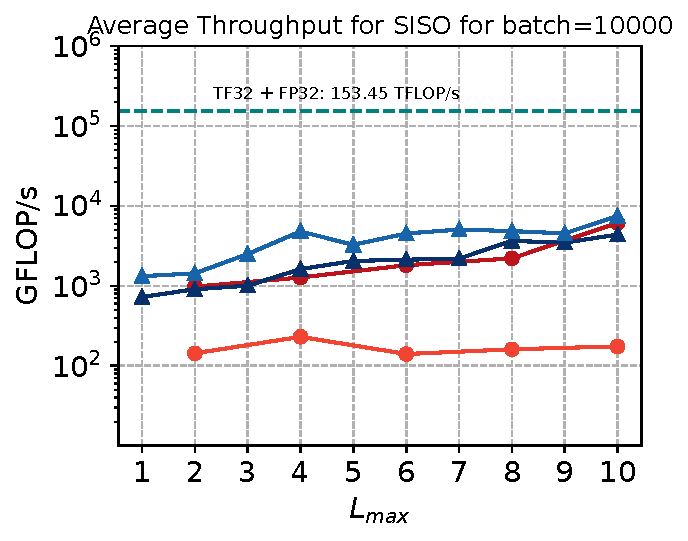
\includegraphics[height=0.16\textheight]
  {figures/ICLR_experiments/mean_all_gflops_SISO_10000_RTX.pdf} &   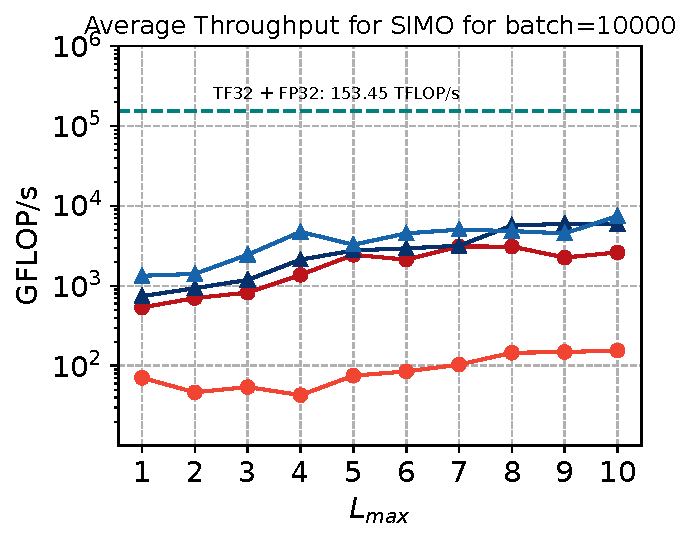
\includegraphics[height=0.16\textheight]{figures/ICLR_experiments/mean_all_gflops_SIMO_10000_RTX.pdf} &  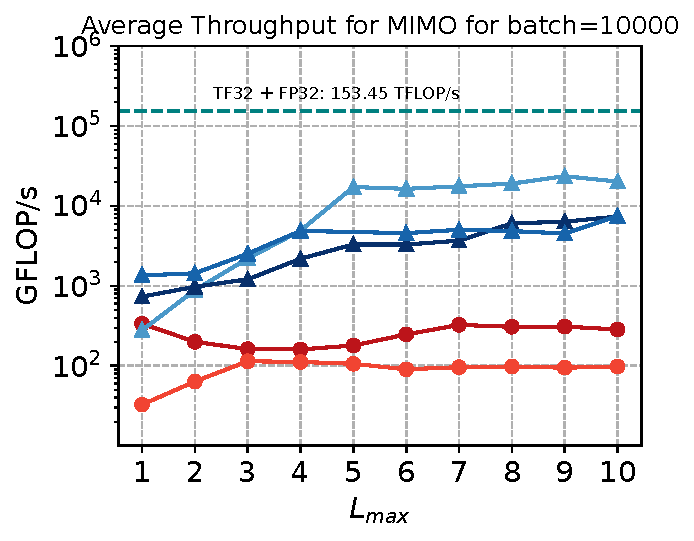
\includegraphics[height=0.16\textheight]{figures/ICLR_experiments/mean_all_gflops_MIMO_10000_RTX.pdf} \\
\end{tabular}
\caption{Analysis of SISO, SIMO and MIMO (\autoref{tab:asymptotic_runtimes} for input settings) performance for different tensor products on RTX A5500 : Total forward walltime (top row),  Total forward normalized walltime (second row), Total GFLOPs   (third row), Total forward normalized GFLOPs (fourth row) and Average forward throughput (bottom row). Note that MTP only supports MIMO. We had to skip values due to profiling errors.}
\label{experiments:benchmarking_gpu_rtx}
\end{figure}

\begin{figure}[!htb]
\begin{tabular}{lll}
  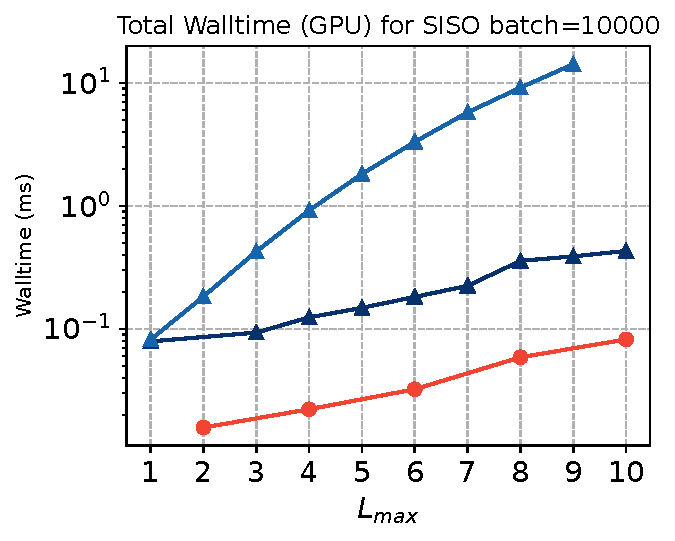
\includegraphics[height=0.16\textheight]{figures/ICLR_experiments/walltime_gpu_SISO_10000_A100.pdf} &   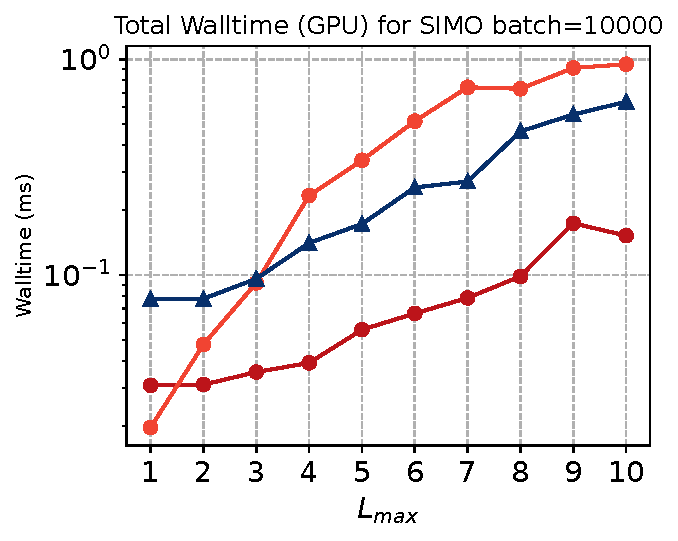
\includegraphics[height=0.16\textheight]{figures/ICLR_experiments/walltime_gpu_SIMO_10000_A100.pdf} &  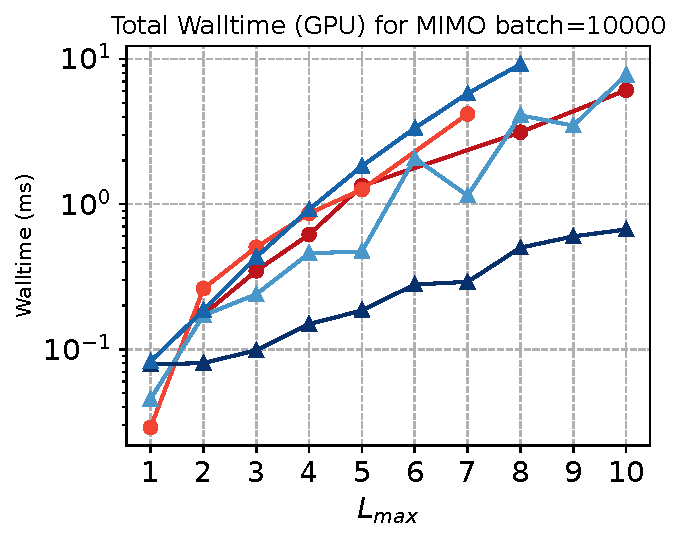
\includegraphics[height=0.16\textheight]{figures/ICLR_experiments/walltime_gpu_MIMO_10000_A100.pdf} \\
  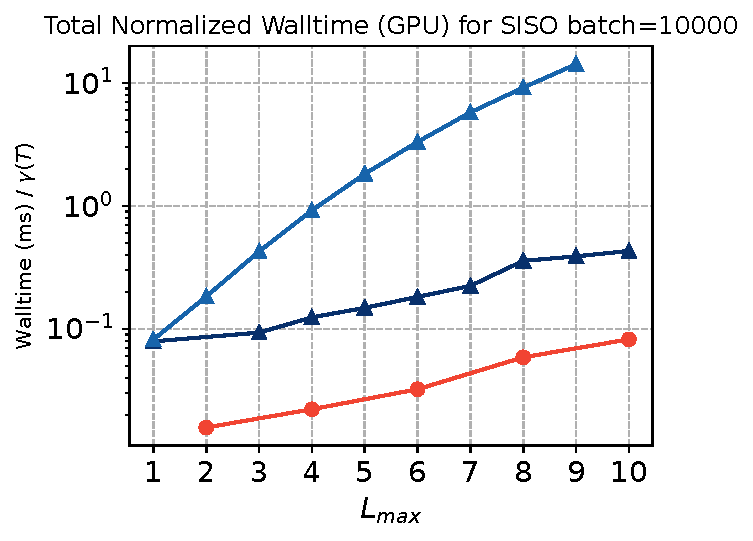
\includegraphics[height=0.16\textheight]{figures/ICLR_experiments/walltime_normalized_gpu_SISO_10000_A100.pdf} &   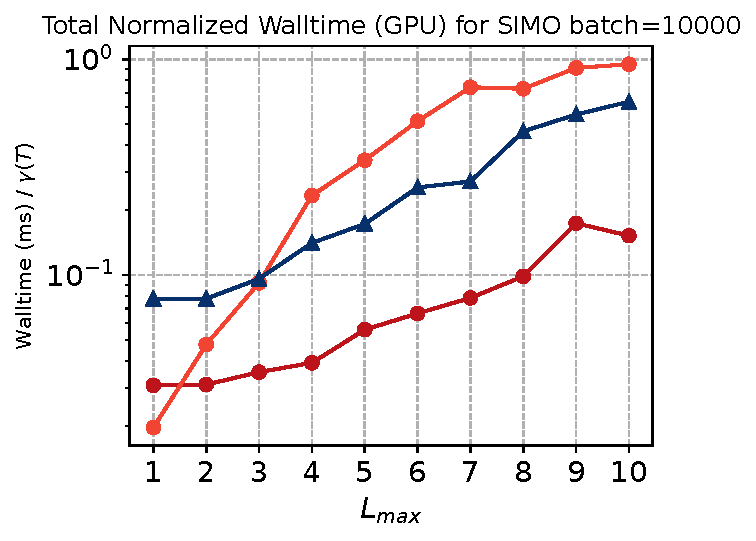
\includegraphics[height=0.16\textheight]{figures/ICLR_experiments/walltime_normalized_gpu_SIMO_10000_A100.pdf} &  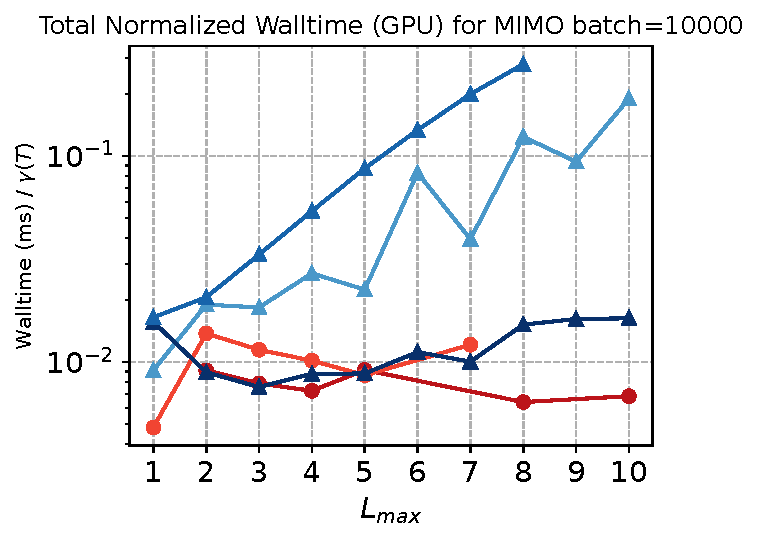
\includegraphics[height=0.16\textheight]{figures/ICLR_experiments/walltime_normalized_gpu_MIMO_10000_A100.pdf} \\
  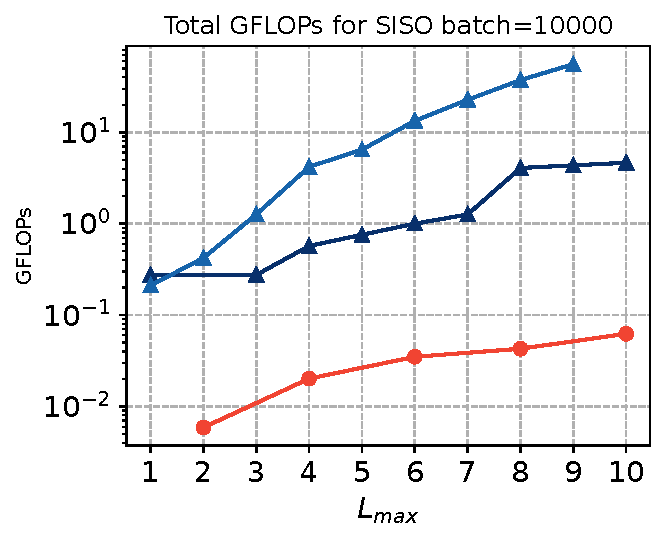
\includegraphics[height=0.16\textheight]{figures/ICLR_experiments/total_all_gflops_SISO_10000_A100.pdf} &   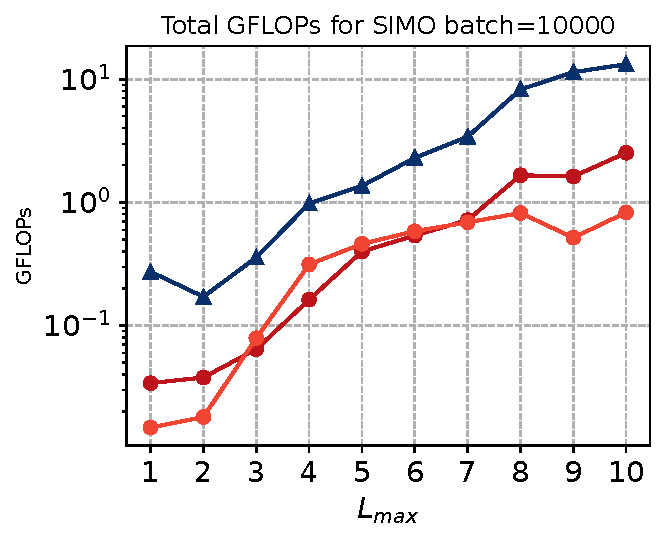
\includegraphics[height=0.16\textheight]{figures/ICLR_experiments/total_all_gflops_SIMO_10000_A100.pdf} &  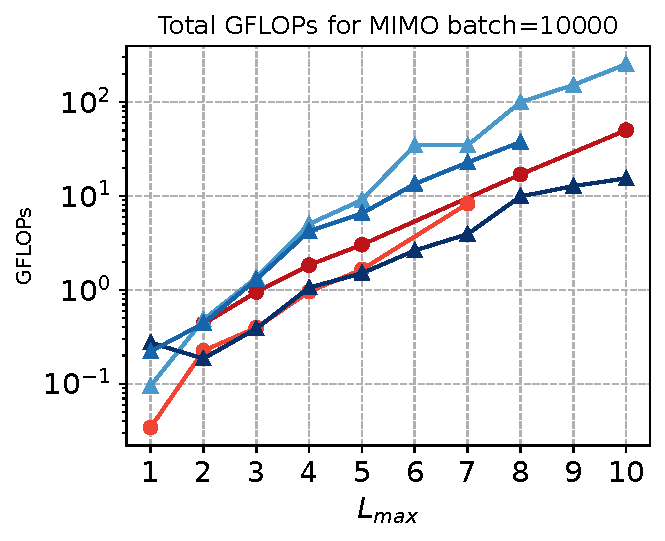
\includegraphics[height=0.16\textheight]{figures/ICLR_experiments/total_all_gflops_MIMO_10000_A100.pdf} \\
  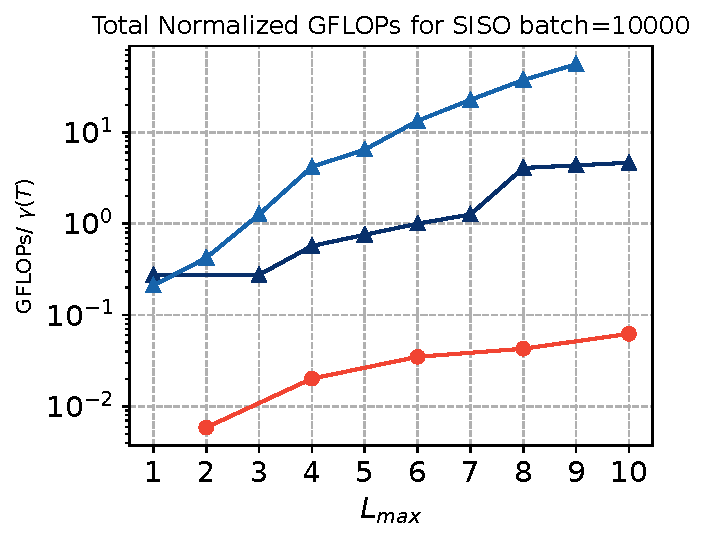
\includegraphics[height=0.16\textheight]{figures/ICLR_experiments/total_normalized_all_gflops_SISO_10000_A100.pdf} &   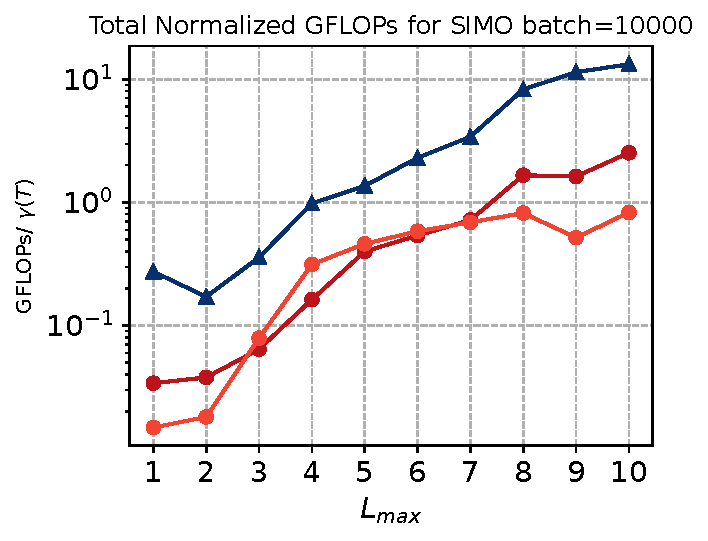
\includegraphics[height=0.16\textheight]{figures/ICLR_experiments/total_normalized_all_gflops_SIMO_10000_A100.pdf} &  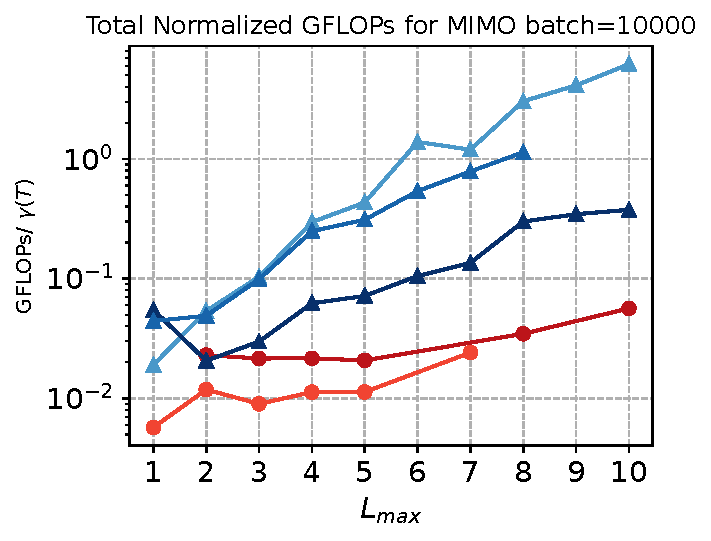
\includegraphics[height=0.16\textheight]{figures/ICLR_experiments/total_normalized_all_gflops_MIMO_10000_A100.pdf} \\
  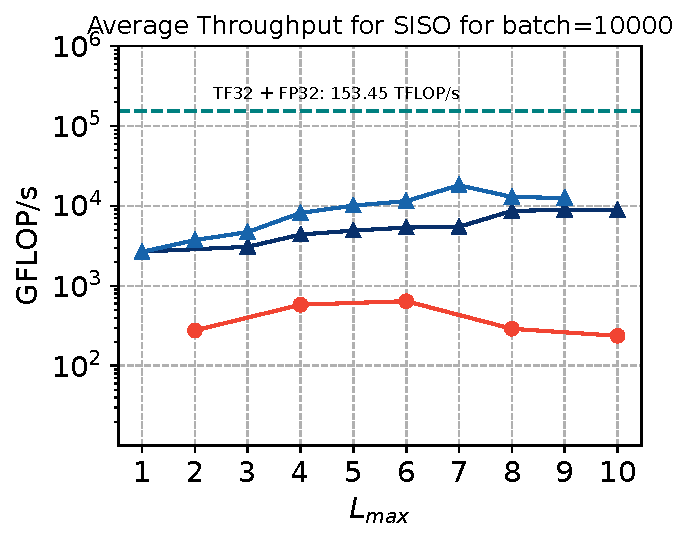
\includegraphics[height=0.16\textheight]
  {figures/ICLR_experiments/mean_all_gflops_SISO_10000_A100.pdf} &   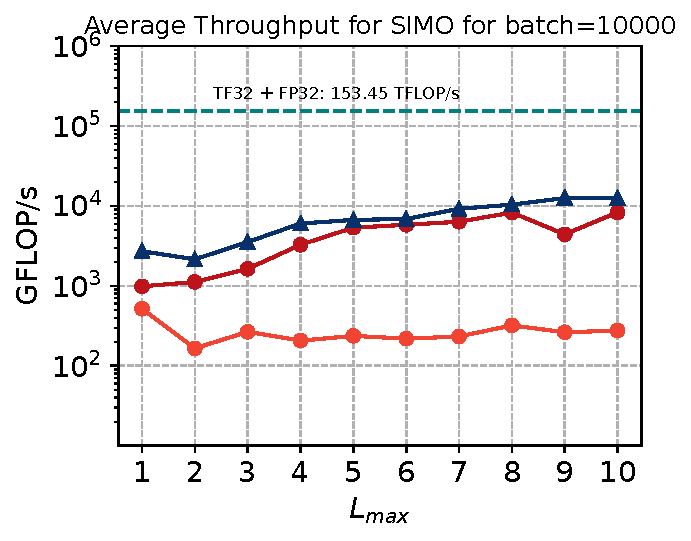
\includegraphics[height=0.16\textheight]{figures/ICLR_experiments/mean_all_gflops_SIMO_10000_A100.pdf} &  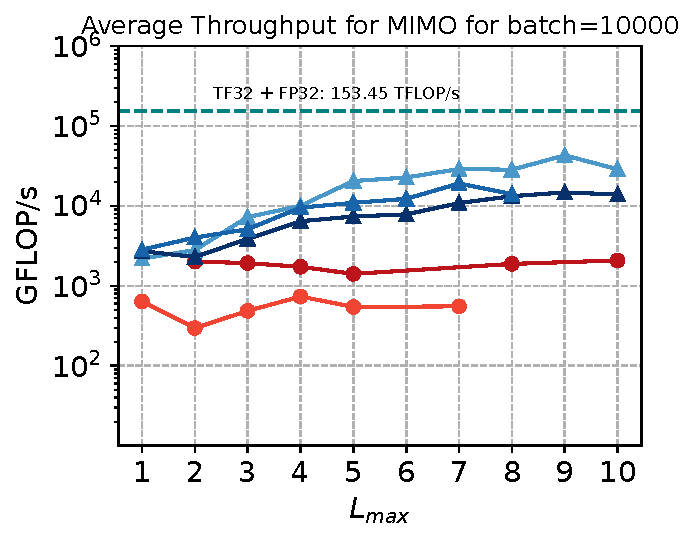
\includegraphics[height=0.16\textheight]{figures/ICLR_experiments/mean_all_gflops_MIMO_10000_A100.pdf} \\
\end{tabular}
\caption{Analysis of SISO, SIMO and MIMO (\autoref{tab:asymptotic_runtimes} for input settings) performance for different tensor products on A100 GPU, showing Total forward walltime (top row),  Total normalized forward walltime (second row), Total forward GFLOPs   (third row) and Total forward normalized GFLOPs (fourth row) and Average forward throughput (bottom row). Note that MTP only supports MIMO. We had to skip values due to profiling errors.}
\label{experiments:benchmarking_gpu_a100}
\end{figure}


\begin{figure}[!htb]
\begin{tabular}{lll}
  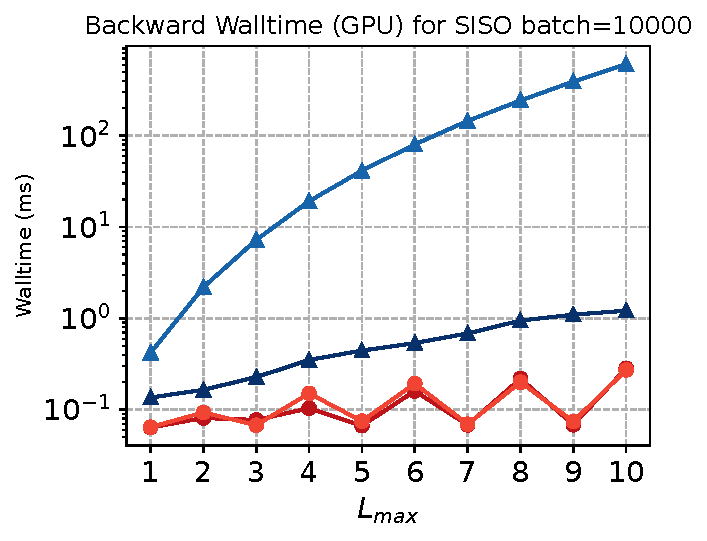
\includegraphics[height=0.16\textheight]{figures/ICLR_experiments/walltime_bwd_gpu_SISO_10000_RTX.pdf} &   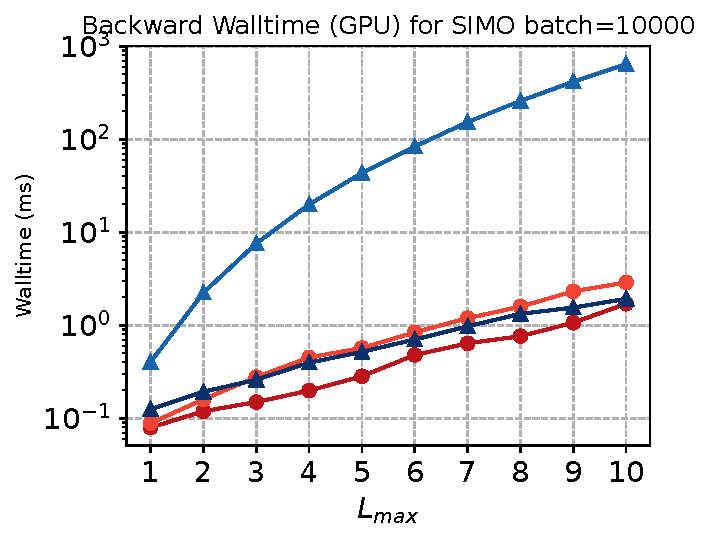
\includegraphics[height=0.16\textheight]{figures/ICLR_experiments/walltime_bwd_gpu_SIMO_10000_RTX.pdf} &  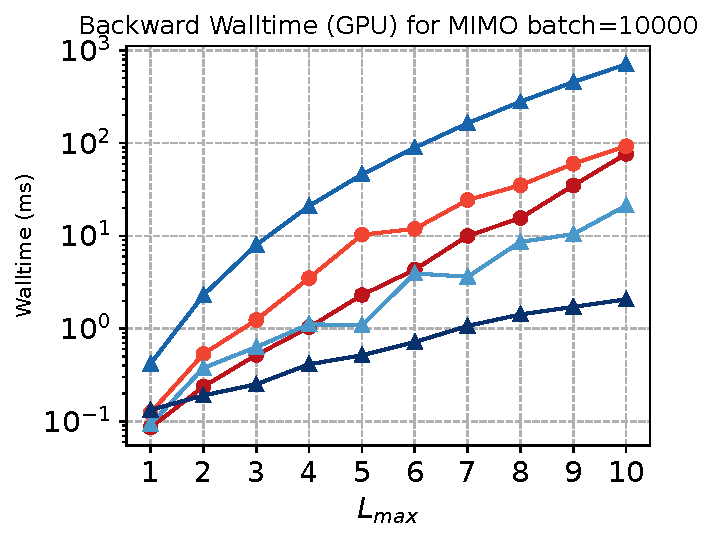
\includegraphics[height=0.16\textheight]{figures/ICLR_experiments/walltime_bwd_gpu_MIMO_10000_RTX.pdf} \\
  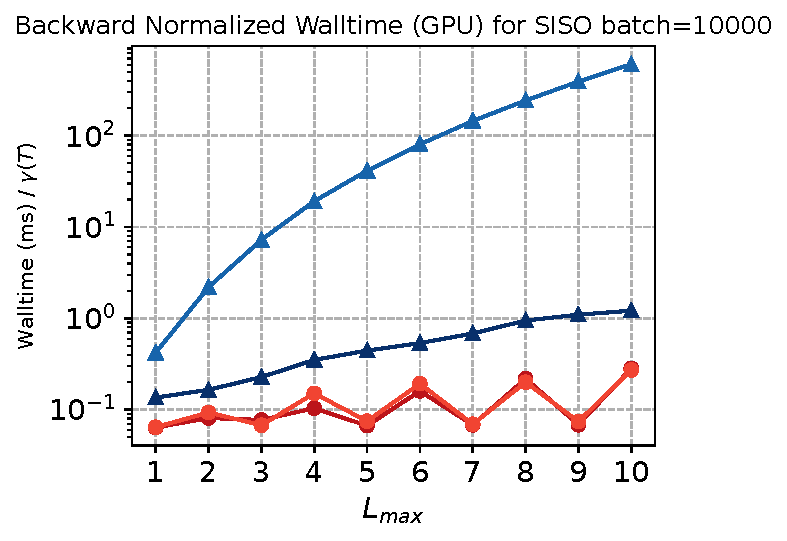
\includegraphics[height=0.16\textheight]{figures/ICLR_experiments/walltime_bwd_normalized_gpu_SISO_10000_RTX.pdf} &   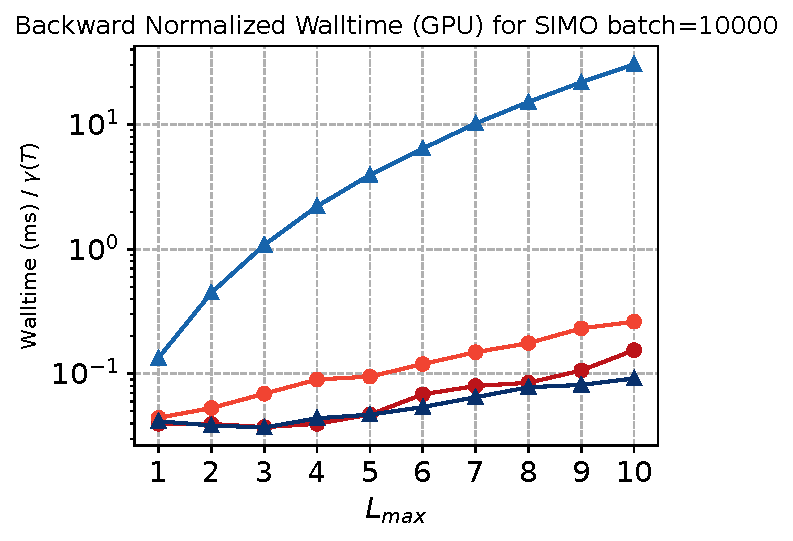
\includegraphics[height=0.16\textheight]{figures/ICLR_experiments/walltime_bwd_normalized_gpu_SIMO_10000_RTX.pdf} &  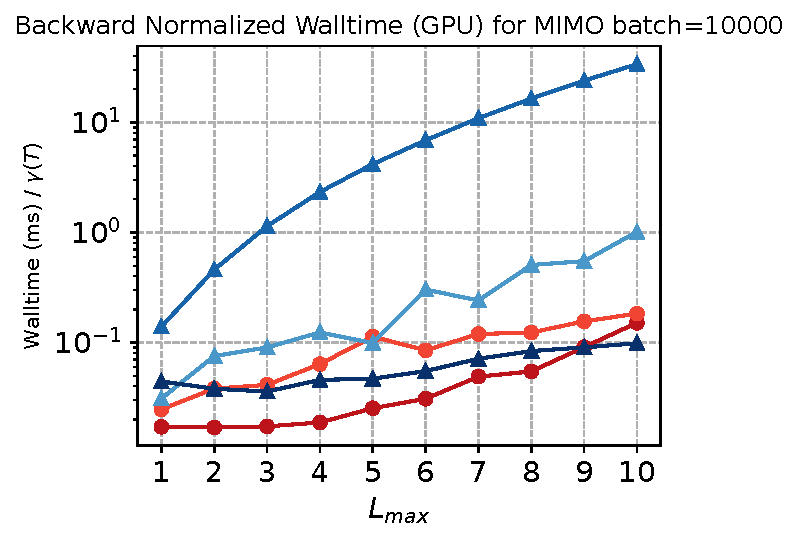
\includegraphics[height=0.16\textheight]{figures/ICLR_experiments/walltime_bwd_normalized_gpu_MIMO_10000_RTX.pdf} \\
\end{tabular}
\caption{Analysis of SISO, SIMO and MIMO (\autoref{tab:asymptotic_runtimes} for input settings) performance for different tensor products on RTX A5500 : Total backward walltime (top row),  Total backward normalized walltime (bottom row). Note that MTP only supports MIMO}
\label{experiments:benchmarking_gpu_bwd_rtx}
\end{figure}